\let\negmedspace\undefined
\let\negthickspace\undefined

\documentclass[journal,12pt,onecolumn]{IEEEtran}
%\documentclass[journal,12pt,twocolumn]{IEEEtran}
%
\usepackage{setspace}
\usepackage{gensymb}
%\doublespacing
\singlespacing

%\usepackage{graphicx}
%\usepackage{amssymb}
%\usepackage{relsize}
\usepackage[cmex10]{amsmath}
%\usepackage{amsthm}
%\interdisplaylinepenalty=2500
%\savesymbol{iint}
%\usepackage{txfonts}
%\restoresymbol{TXF}{iint}
%\usepackage{wasysym}
\usepackage{amsthm}
\usepackage{mathrsfs}
\usepackage{txfonts}
\usepackage{stfloats}
\usepackage{cite}
\usepackage{cases}
\usepackage{subfig}
%\usepackage{xtab}
\usepackage{longtable}
\usepackage{multirow}
%\usepackage{algorithm}
%\usepackage{algpseudocode}
\usepackage{enumitem}
\usepackage{mathtools}
\usepackage{tikz}
\usepackage{circuitikz}
\usepackage{verbatim}
\usepackage{hyperref}
%\usepackage{stmaryrd}
\usepackage{tkz-euclide} % loads  TikZ and tkz-base
%\usetkzobj{all}
\usepackage{listings}
\usepackage{color}                                            %%
\usepackage{array}                                            %%
\usepackage{longtable}                                        %%
\usepackage{calc}                                             %%
\usepackage{multirow}                                         %%
\usepackage{hhline}                                           %%
\usepackage{ifthen}                                           %%
%optionally (for landscape tables embedded in another document): %%
\usepackage{lscape}     
\usepackage{multicol}
\usepackage{chngcntr}
\usepackage{iftex}
%\usepackage[latin9]{inputenc}
\usepackage{geometry}
\usepackage{bm}
%\geometry{verbose,tmargin=2cm,bmargin=3cm,lmargin=1.8cm,rmargin=1.5cm,headheight=2cm,headsep=2cm,footskip=3cm}
\usepackage{array}
\newcolumntype{L}[1]{>{\raggedright\let\newline\\\arraybackslash\hspace{0pt}}m{#1}}
\newcolumntype{C}[1]{>{\centering\let\newline\\\arraybackslash\hspace{0pt}}m{#1}}
\newcolumntype{R}[1]{>{\raggedleft\let\newline\\\arraybackslash\hspace{0pt}}m{#1}}

%\usepackage{graphicx}
%\usepackage{setspace}
%\usepackage{parskip}

\def \hsp {\hspace{3mm}}

\makeatletter

\providecommand{\tabularnewline}{\\}



\makeatother
\ifxetex
\usepackage[T1]{fontenc}
\usepackage{fontspec}
%\setmainfont[ Path = fonts/]{Sanskrit_2003.ttf}
\newfontfamily\nakulafont[Script=Devanagari,AutoFakeBold=2,Path = fonts/]{Nakula}
%\newfontfamily\liberationfont{Liberation Sans Narrow}
%\newfontfamily\liberationsansfont{Liberation Sans}
\fi
\usepackage{tikz}
\usepackage{xcolor}
%\usepackage{enumerate}

%\usepackage{wasysym}
%\newcounter{MYtempeqncnt}
\DeclareMathOperator*{\Res}{Res}
%\renewcommand{\baselinestretch}{2}
\renewcommand\thesection{\arabic{section}}
\renewcommand\thesubsection{\thesection.\arabic{subsection}}
\renewcommand\thesubsubsection{\thesubsection.\arabic{subsubsection}}

\renewcommand\thesectiondis{\arabic{section}}
\renewcommand\thesubsectiondis{\thesectiondis.\arabic{subsection}}
\renewcommand\thesubsubsectiondis{\thesubsectiondis.\arabic{subsubsection}}

% correct bad hyphenation here
\hyphenation{op-tical net-works semi-conduc-tor}
\def\inputGnumericTable{}                                 %%

\lstset{
	language=tex,
	frame=single, 
	breaklines=true
}

%\begin{document}
%


\newtheorem{theorem}{Theorem}[section]
\newtheorem{problem}{Problem}
\newtheorem{proposition}{Proposition}[section]
\newtheorem{lemma}{Lemma}[section]
\newtheorem{corollary}[theorem]{Corollary}
\newtheorem{example}{Example}[section]
\newtheorem{definition}[problem]{Definition}
%\newtheorem{thm}{Theorem}[section] 
%\newtheorem{defn}[thm]{Definition}
%\newtheorem{algorithm}{Algorithm}[section]
%\newtheorem{cor}{Corollary}
\newcommand{\BEQA}{\begin{eqnarray}}
	\newcommand{\EEQA}{\end{eqnarray}}
\newcommand{\define}{\stackrel{\triangle}{=}}
\bibliographystyle{IEEEtran}
%\bibliographystyle{ieeetr}
\providecommand{\mbf}{\mathbf}
\providecommand{\pr}[1]{\ensuremath{\Pr\left(#1\right)}}
\providecommand{\qfunc}[1]{\ensuremath{Q\left(#1\right)}}
\providecommand{\sbrak}[1]{\ensuremath{{}\left[#1\right]}}
\providecommand{\lsbrak}[1]{\ensuremath{{}\left[#1\right.}}
\providecommand{\rsbrak}[1]{\ensuremath{{}\left.#1\right]}}
\providecommand{\brak}[1]{\ensuremath{\left(#1\right)}}
\providecommand{\lbrak}[1]{\ensuremath{\left(#1\right.}}
\providecommand{\rbrak}[1]{\ensuremath{\left.#1\right)}}
\providecommand{\cbrak}[1]{\ensuremath{\left\{#1\right\}}}
\providecommand{\lcbrak}[1]{\ensuremath{\left\{#1\right.}}
\providecommand{\rcbrak}[1]{\ensuremath{\left.#1\right\}}}
\theoremstyle{remark}
\newtheorem{rem}{Remark}
\newcommand{\sgn}{\mathop{\mathrm{sgn}}}
\providecommand{\abs}[1]{\left\vert#1\right\vert}
\providecommand{\res}[1]{\Res\displaylimits_{#1}} 
\providecommand{\norm}[1]{\left\lVert#1\right\rVert}
%\providecommand{\norm}[1]{\lVert#1\rVert}
\providecommand{\mtx}[1]{\mathbf{#1}}
\providecommand{\mean}[1]{E\left[ #1 \right]}
\providecommand{\fourier}{\overset{\mathcal{F}}{ \rightleftharpoons}}
%\providecommand{\hilbert}{\overset{\mathcal{H}}{ \rightleftharpoons}}
%\providecommand{\system}{\overset{\mathcal{H}}{ \longleftrightarrow}}
\providecommand{\system}[1]{\overset{\mathcal{#1}}{ \longleftrightarrow}}
\providecommand{\gauss}[2]{\mathcal{N}\ensuremath{\left(#1,#2\right)}}
%
%\newcommand{\solution}[2]{\textbf{Solution:}{#1}}
\newcommand{\solution}{\noindent \textbf{Solution: }}
\newcommand{\cosec}{\,\text{cosec}\,}
\newcommand{\sinc}{\,\text{sinc}\,}
\newcommand{\rect}{\,\text{rect}\,}
\providecommand{\dec}[2]{\ensuremath{\overset{#1}{\underset{#2}{\gtrless}}}}
\newcommand{\myvec}[1]{\ensuremath{\begin{pmatrix}#1\end{pmatrix}}}
\newcommand{\mydet}[1]{\ensuremath{\begin{vmatrix}#1\end{vmatrix}}}
\newcommand*{\permcomb}[4][0mu]{{{}^{#3}\mkern#1#2_{#4}}}
\newcommand*{\perm}[1][-3mu]{\permcomb[#1]{P}}
\newcommand*{\comb}[1][-1mu]{\permcomb[#1]{C}}
%\numberwithin{equation}{section}
\numberwithin{equation}{section}
%\numberwithin{problem}{section}
%\numberwithin{definition}{section}
\makeatletter
\@addtoreset{figure}{problem}
\makeatother
%\let\StandardTheFigure\thefigure
\let\vec\mathbf
%\renewcommand{\thefigure}{\theproblem.\arabic{figure}}
\renewcommand{\thefigure}{\arabic{section}.\arabic{figure}}
%\setlist[enumerate,1]{before=\renewcommand\theequation{\theenumi.\arabic{equation}}
	%\counterwithin{equation}{enumi}
	%\renewcommand{\theequation}{\arabic{subsection}.\arabic{equation}}
\let\StandardTheFigure\thefigure
	\vspace{3cm}
	%\usepackage{babel}
	\begin{document}
	  \title{K-means}
	  \author{ Mannem Charan AI21BTECH11019}
          \maketitle
	   \begin{abstract}
		This report consists of my basic understanding of one of the popular Ml methods "K-means Clustering".
	   \end{abstract}
           \section{K-means}
            K-means or K-means clustering algorithm is used to solve the clustering problem. It comes under unsupervised machine learning, where the data don't have any labels.
	   \section{What is Clustering Problem?}
	     Often it happens the we don't have labels for the data.So in those cases we try to divide the data into different groups intuitively.For example see the figure $\ref{Fig 1}$, we are trying to group the data points which are close to each other.\\
	     \begin{figure}
	       \centering
	       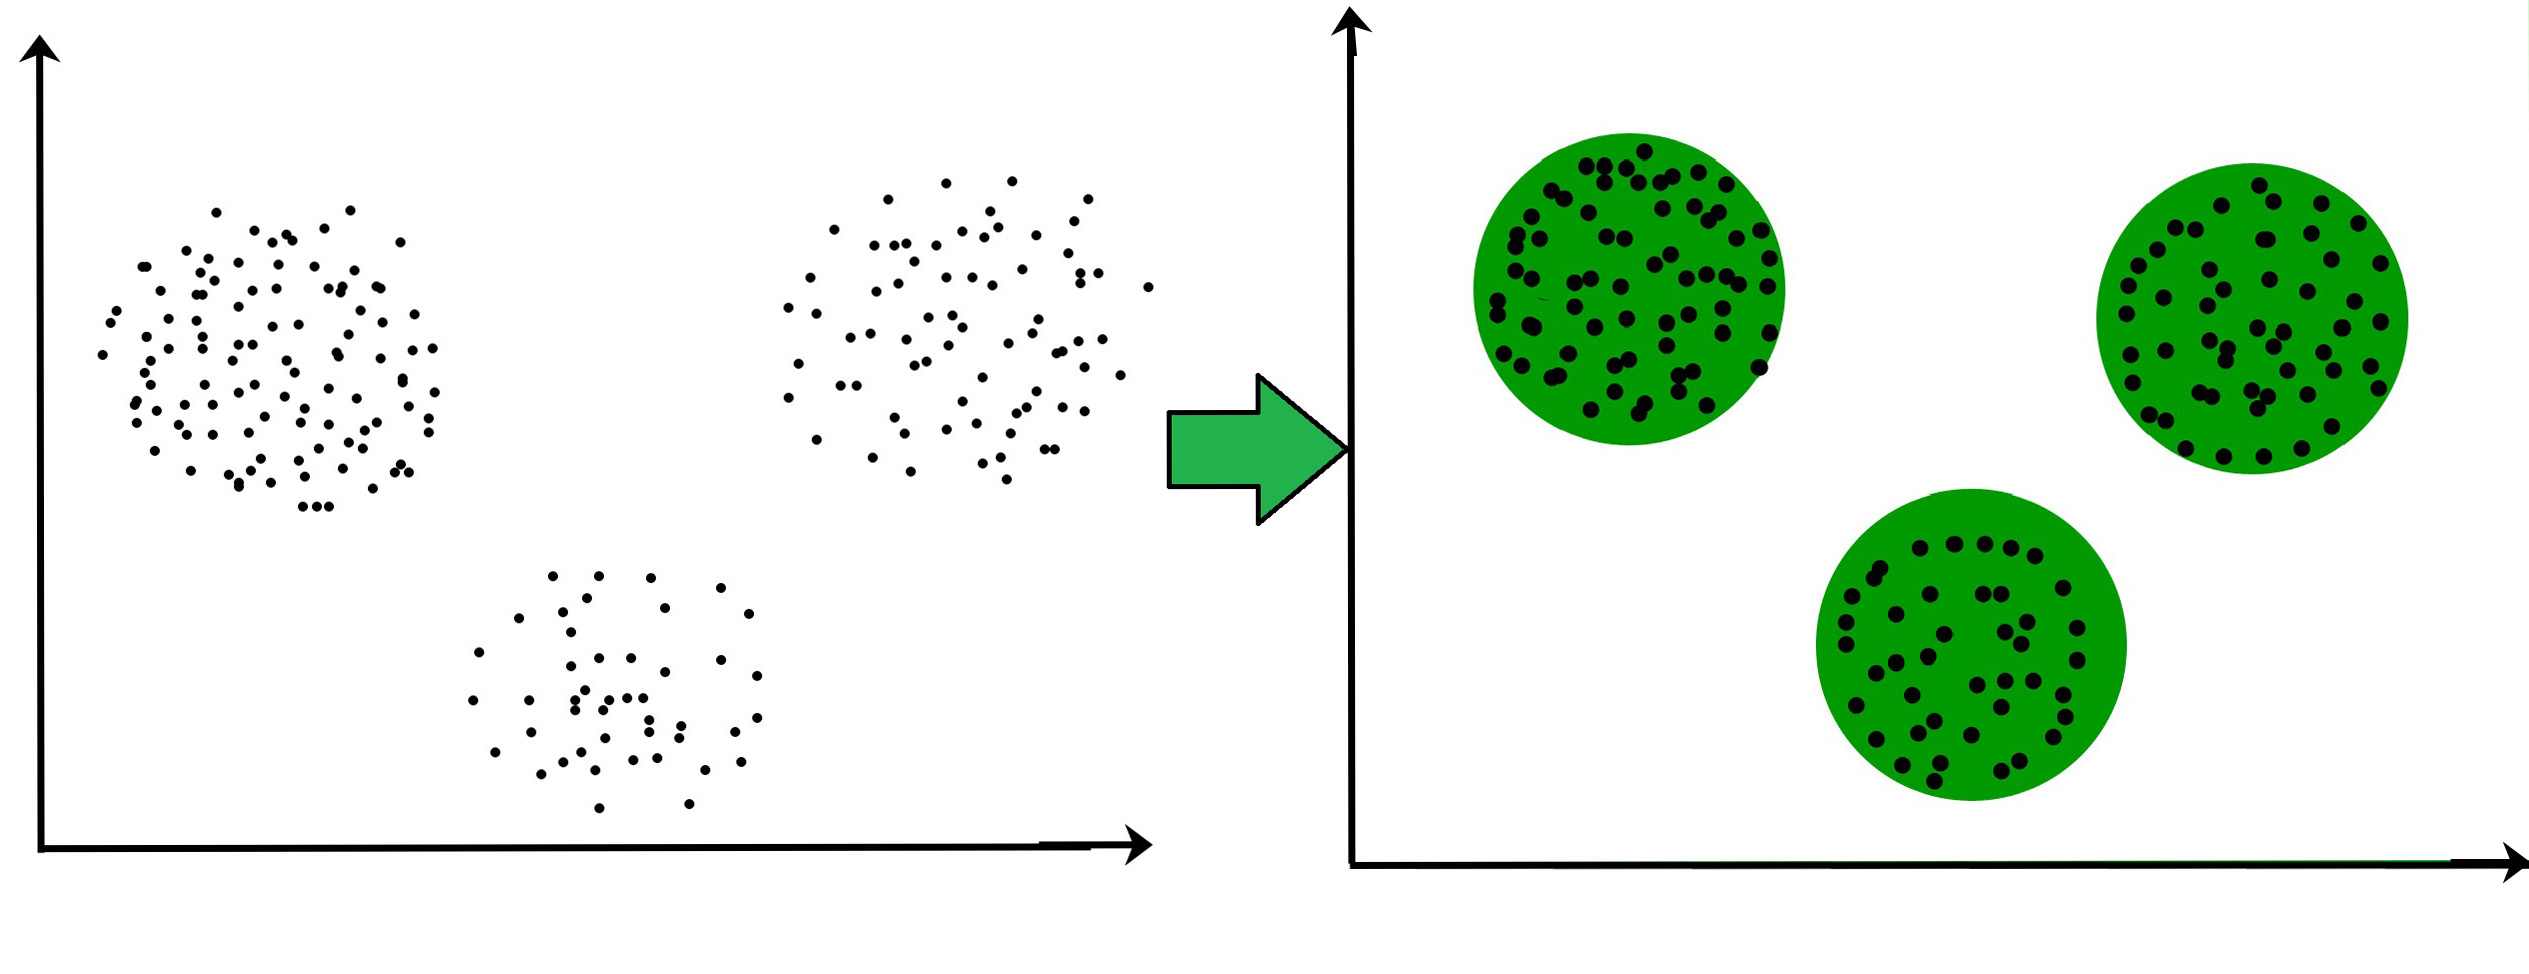
\includegraphics[width = 10cm]{clustering.jpg}
	       \caption{An example of grouping/clustering}
	       \label{Fig 1}
	      \end{figure}
         These groups are known as "Clusters". And this process of grouping is known as "Clustering".
	    \section{Understanding K-means Clustering}
            In the k-means algorithm, we will try to divide the data set into "k" clusters and a data point will become member of a cluster if it closest to that cluster in comparison to other clusters.It is kinda similar to k-NN algorithm but there the data we use have some pre-defined labels but here we are just trying to seperate the data into groups/clusters. The word "means" represent center of the each cluster.And we want to make sure that each point in a Cluster say $A$ should be closest to the mean of $A$ than the means of other clusters.In practice, the algorithm is done by following steps,
		    \begin{enumerate}
			\item First we will intialise the value of "k", the number of clusters we want to make from the data.
		        \item Now we should generate k centers of clusters but initially we can't find the exact position of centers of the clusters.So we will generate "k" points randomly.
		        \item Since we initialised the mean points, we will assign the data points to each mean point depending how close they are to the mean point.To find "closeness" between data points and mean points we will use euclidean distance metric,
				\begin{align}
					d\brak{\vec{x},\vec{c}} &= \sqrt{\sum_{i=1}^{n}\brak{x_i-c_i}^2}
				\end{align}
				    where,
				\begin{itemize}
					\item $\vec{x}$ = data point
					\item $\vec{c}$ = mean/centroid point
					\item $\vec{n}$ = no. of features.
				\end{itemize}
			So for every data point we will find the closest mean point and assign the point to that cluster.
			 \item Then we will update the mean point of the cluster as the average of all the data points in that cluster.So the new mean point will be,
				  \begin{align}
					  \vec{c'} &= \frac{1}{N}\sum_{i=1}^{N}\vec{x_i}
			          \end{align}
				    where,
				    \begin{itemize}
					 \item $\vec{c'}$ = new mean point of the cluster
					 \item N = The no. of data points in the cluster.
					 \item $\vec{x_i}$ = $i^{th}$ data point in the cluster.
				    \end{itemize}
			 \item Then repeat the step 3 and 4 until there is no change in the grouping of clusters.
		      \end{enumerate}
	     \section{Advantages of k-means}
		     \begin{enumerate}
		       \item It is easy to implement.
		       \item One of the preffered methods if the dataset is large and don't pre-defined labels.
		       \item Guarantees the convergence.
	             \end{enumerate}
	     \section{Disadvantages of k-means}
		      \begin{enumerate}
		       \item Uses lot of computational power.
		       \item Asks the user to give the "k" value, can be resolved by plotting the squared error vs k curve.
		       \item Mean points can be dragged near to outlier points or outliers might get their own clusters instead of being ignored.
		       \item Causes problems for high-dimensional data because the distance measure will not be effective to seggregate the clusters.
	              \end{enumerate}
	     \section{Questions}
		     \begin{enumerate}
		       \item Which part of machine learning k-means algorithm belongs to?
		       \item What is a cluster?
		       \item What is the difference betweeen the k-means and k-NN algorithms?
		       \item What are the challenges in k-means algorithm?
		       \item How the optimal k can be found for the given data?
	              \end{enumerate}
	     \section{Solution}
		     \begin{enumerate}
		       \item k-means algorithm can under unsupervised learning where input data doesnot have pre-defined labels.
		       \item In machine learning, cluster is group of data points having some similarities.
		       \item 
			      \begin{itemize}
			        \item k-means algorithm used for unsupervised learning whereas k-NN is used for supervied learning.
			        \item The k in k-means represents the number of clusters to be grouped in the data whereas in k-NN it represents the no. of closest number you want to consider to classify the data.
			        \item In k-means we want to \textbf{group} the data based on how close the points are , whereas in k-NN we try to \textbf{classify} a data point to a class based on majority in neighbours.
				\item K-means often has outliers problems whereas it can be resolved in k-NN by taking higher values of k.
			      \end{itemize}
		       \item The main challenges in k-means algorithm are,
			       \begin{itemize}
				 \item Choosing the value of $k$.
			         \item Generating the $k$ centroids/mean points.
			       \end{itemize}
		       \item The optimal $k$ can be found for a given data using elbow method.In this method we try to plot within-cluster sum squared error$\brak{WSS}$ against different values of k. The sharp point of bend or the point where it looks like elbow, that point will be our optimal $k$ value.The WSS is formulated as,
			        \begin{align}
					WSS &= \sum_{j=1}^{k}\sum_{i=1}^{N_j}\norm{\vec{x_i^{\brak{j}}} -\vec{C_j}}^{2}
			        \end{align}
				     where,
				     \begin{itemize}
				       \item k = no. of clusters
				       \item $\vec{C_j}$ = centroid of $j^{th}$ cluster.
				       \item $N_j$ = no. of samples in $j^{th}$ cluster.\\
				       \item $\vec{x_i^{\brak{j}}}$ =  $i^{th}$ data point of $j^{th}$ cluster.
				     \end{itemize}
		We are taking the point where there is abrupt decrease because we want to make the centroid as close as possible to the all the points in the cluster.
		      \end{enumerate}
         \end{document}     
